%! TEX root = ../aminhash.tex

\section{The Estimators}

In this section we develop a maximum likelihood estimator (MLE) for MinHash, analyse the variance and compare it to the classical MinHash estimator.
Such an estimator has the lower possible variance asymptotically as $K\to\infty$, but it is slow to evaluate, which destroys the gains from needing fewer MinHash values.
We thus proceed to develop a third estimator that is as fast as the classical estimator.
We call it the Minner estimator and we show experimentally that it requires nearly as few MinHash values as the MLE for equivalent recall.
In fact, for $K < 50$ it requires fewer values than even the MLE.

A quick note on notation: If $u\in\mathbb N$, we use $[u]=\{0,\dots,u-1\}$ to indicate the set of numbers up to $u$.
If $P$ is a proposition, we use $[P]$ to indicate the variable that is $1$ if $P$ and $0$ if not $P$.

\subsection{Maximum Likelihood Estimator}

Given a random variable and a statistical model, ``estimation'' is the task of inferring the parameters to the model on the basis of the observation.
A maximum likelihood estimator chooses the parameters that maximizes the probability that the model generates the particular observed value.
That is, if the observation is equal to $\rho$ with probability $p(\rho;\,\theta)$, $\theta$ is unknown, once we observe $\rho$, we estimate $\theta$ as the $\argmax p(\rho;\,\theta)$.

% A statistical model for a MLE contains four types of variables:
% Those we know at the time of estimation;
% those that are random but we observe;
% those that are random and hidden;
% and those we want to estimate.

In our case we get the following model:
Given a set $X$, a hash function $h:U\to [0,1]$, and values $n_y$ and $v$, we sample a set $Y\subseteq U$ with $|Y|=n_y$ and $v=|X\cap Y|$.
We let $r$ be the smallest value $h(y)$ for $y\in Y$.
The log-likelihood of the observation is then:
\[
   \ell(r; v) = \log\Pr_{Y}[\min_{y\in Y}h(y) = r].
\]
We note a couple of things about the model:
1) By assuming $Y$ is generated uniformly at random among sets of size $n_y$ and overlap $v$ we are making a specific choice that may not be optimal for all datasets.
In the ``skewed data'' model of~\cite{mccauley2018set} a Bayesian might incorporate a particular presumption about the sets $Y$ and increase the precision of the estimator.
2) We can get the same model by taking $Y$ to be known, but the hash values $h(y)$ to be unknown.
This is more similar to the classical MinHash analysis, but doesn't make a big difference in our case, except by making it harder to be a Bayesian.
3) If we do not consider $n_y$ to be known, we can let the model have two parameters and estimate both of them.
We could for example count the frequency of set sizes in the database and build this into the model, however in the database model we might as well just store the set sizes and use them directly.

As a first step to computing $\ell(r;v)$ we not that $h$ can be assumed to take values in $[u]$ rather than $[0,1]$ and a be a bijection.
However then $h$ simply represents a known permutation of $[u]$ and we can ignore it all together.
Then the observed MinHash value is the random variable $R=\min_{y\in Y} y$.
We define $n_x = |X|$, and $M = \sum_{x\in X} [x < R]$ to be the number of ``minner values'' -- a random variable which is a function of $R$.
We proceed to prove the following proposition:
\begin{proposition}
   Let $r\in[u]$ be the MinHash of $Y$ and let $y^*$ (also $\in[i]$) be its index such that $h(y^*)=r$.
   Let $m=m(r)=\sum_{x\in X}[x < r]$ then
\[
   \Pr_Y[R=r]
    =
    \begin{cases}
      \frac{\binom{n_x-m-1}{v-1}\binom{u-r-(n_x-m)}{n_y-v}}{\binom{n_x}{v}\binom{u-n_x}{n_y-v}}
      &
      \text{if $y^*\in X$, and}
       \\
      \frac{\binom{n_x-m}{v}\binom{u-r-1-(n_x-m)}{n_y-v-1}}{\binom{n_x}{v}\binom{u-n_x}{n_y-v}}
      & \text{if $y^*\not\in X$}
    \end{cases}
 \]
 \label{prop:prob}
\vspace{-1em} %Some weird spacing going on here.
\end{proposition}
Note we take $\binom{n}{k}=0$ for $n<k$.
In particular this may happen if $n_x-m<v$.
The probability of $R=r$ in this case is 0, since $n_x-m$ is the number of x-ranks at least $r$, and all of $X\cap Y$ must have rank at least $r$.
\begin{proof}
   Not considering $R$ there are $\binom{n_x}{v}\binom{u-n_x}{n_y-v}$ ways to choose $Y$ such that $|Y|=n_y$ and $|X\cap Y|=v$.
   We proceed by cases..

   First consider the case $r\in X$.
   Then the remaining $v-1$ overlapping elements have to be chosen from $\{x\in X:x > r\}$.
   by definition of $m$ there are $n_x-m-1$ such values.
   The remaining $n_y-v$ non-overlapping elements have to be chosen from $\{x\not\in X: x > r \}$.
   There are $u-r$ elements in $[u]$ greater than $r$, and of those $n_x-m$ are in $X$.
   Thus the number of ways to choose $Y$ with $r\in X$ is
   $\binom{n_x-m-1}{v-1}\binom{u-r-(n_x-m)}{n_y-v}$.

   The case $r\not\in X$ follows by similar arguments.
\end{proof}

Using \cref{prop:prob} we can write the log-likelihood in the following concise manner:
\[
   \ell(r; v) = \log \frac{\binom{n_x-m-[r\in X]}{v-[r\in X]}\binom{u-r-[r\not\in X]-(n_x-m)}{n_y-v-[r\not\in X]}}{\binom{n_x}{v}\binom{u-n_x}{n_y-v}}.
   \label{eq:log-likelihood}
\]
If we observe $K>1$ values $r_1, r_2, \dots, r_K$ we get, by independence of the MinHash functions, a log likelihood of
\[
   \ell(r_1; v) + \ell(r_2; v) + \dots + \ell(r_K; v).
\]
It is trivial to enumerate all $v\in[\min\{n_x,n_y\}+1]$ and compute which one has the highest log-likelihood.
\begin{definition}[Maximum Likelihood Estimator (MLE)]
   The maximum likelihood estimators for respectively set overlap and Jaccard similarity are
   \begin{align}
      T_v(r_1,\dots,r_K) &= \argmax_{v\in[\min\{n_x,n_y\}+1]} \ell(r_1; v) + \ell(r_2; v) + \dots + \ell(r_K; v).
      \\T_j(r_1,\dots,r_K) &= \frac{T_v(r_1,\dots,r_K)}{n_x+n_y - T_v(r_1,\dots,r_K)}.
   \end{align}
\end{definition}
%
The definition gives our first estimator.

\subsection{Analysis}

We want to analyse the MLE estimator in the model where $h$ is unknown.
In this setting we know that the variance of the classical MinHash estimator is
\[
   \frac{E[(T-j)^2]}{K}
      = \frac{E[T^2] - j^2}{K}
      = \frac{\Pr[T=1] - j^2}{K}
      = \frac{j(1-j)}{K}.
      \label{eq:minvar}
\]
This is important because we want to know the general expected performance of the algorithm, and not what it does after some particular random event.

TODO: We should talk about bias before variance.

The main work of this section will be proving the following proportion:
\begin{proposition}\label{prop:mle_var}
   As $K\to\infty$, the variance of the MLE estimator converges to
   \[
      \frac{j (1+j)^3 n_y (n_y-j n_x) (n_x-j n_y)}{(n_x+n_y) \left((1+j)^2 n_xn_y - j^2 (n_x+n_y)^2\right)K}
   \label{eq:mle_var}
   \]
   over the randomness of the random hash function.
\end{proposition}

\begin{figure}
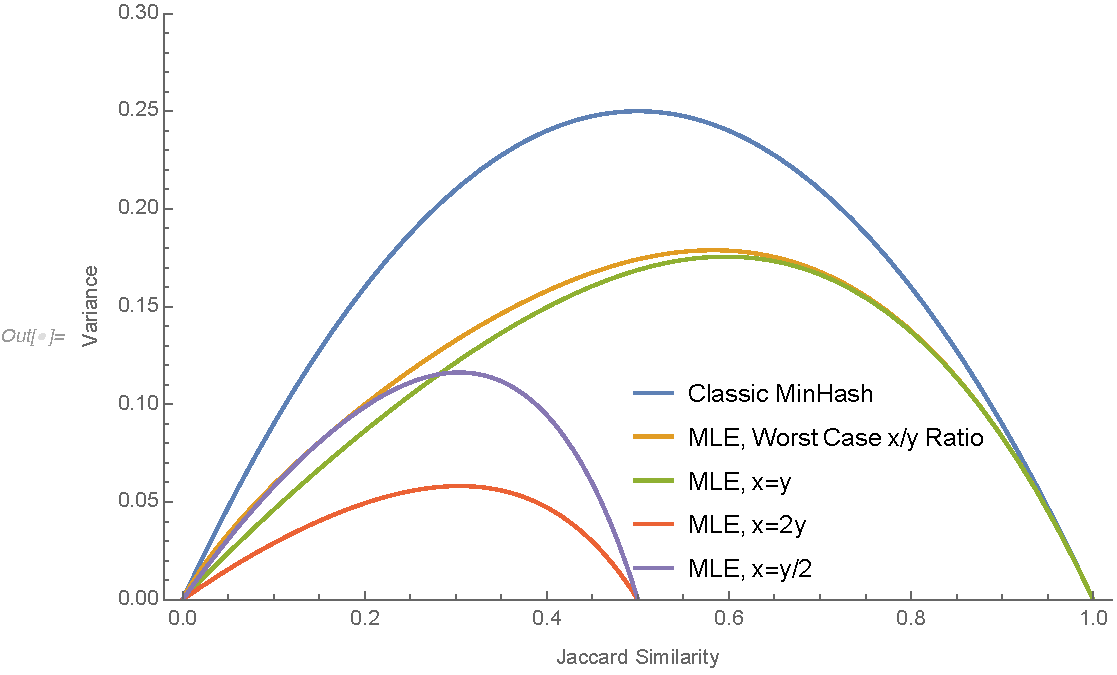
\includegraphics[trim=30 0 0 0,clip,width=\linewidth]{figures/mle_variance2}
\caption{Variance of maximum likelihood estimator based on Fischer Information bound.
For $j$ close to 0 or 1 the worst case MLE bound is asymptotically equal to the Classical bound, whereas for $j\approx 0.21$ has only $\approx 62\%$ of the variance.
See \cref{fig:exp_variance} for a corresponding experimental test.
}
\label{fig:mle_variance}
\end{figure}

The bound is a little complicated by the fact that it includes the sizes of the sets $n_x$ and $n_y$.
We note that the bound is convex in the ratio $n_y/n_x$, giving lower variances than \cref{eq:minvar} for $n_x<\!<n_y$ or $n_x >\!> n_y$.
\Cref{fig:mle_variance} shows \cref{eq:mle_var} when the ratio is taken to be \emph{worst possible}, as well as when it is taken to be 1
In the symmetric case $n_x=n_y$ the asymptotic variance reduces to
\[
   \frac{j(1-j)}{K}\frac{(1+j)^3}{2(1+3j)}.
\]
%for large $x$ and $y$.
For $n_x/n_y\neq1$ the Jaccard similarity is bounded above by $\frac{\min\{n_x,n_y\}}{\max\{n_x,n_y\}}$, which allows the MLE to discard those higher values from consideration.
Another interesting point from \cref{eq:mle_var} is that the variance at $n_x=c n_y$ is exactly $1/c$ of the variance at $n_x=n_y/c$.
It makes sense that the variance is lower when $|X|$ is big compared to $|Y|$, since we are given $X$, but don't know $Y$.

TODO: Stuff about local/global risk.
We can also compute the global risk of the MLE estimator, which is $0.178847/K$, $28.5\%$ less than the Classical Estimator.

\begin{proof}[Proof of \cref{prop:mle_var}]
   We first find the variance for the MLE estimator for $v$ and then show how to re-parametrize it to use the Jaccard similarity.

   Using Stirling's approximation $ \log n! = n\log n - n + O(\log n)$,
   we rewrite the log-likelihood \cref{eq:log-likelihood} as
   \begin{align}
      \ell(r;v) &=
      (x-k-[y^*\in X]+1)H(\tfrac{v-[y^*\in X]}{x-k-[y^*\in X]+1})
               - (x+1) H(\tfrac{v}{x+1})
              \\&+(u-m-[y^*\not\in X]-x+k+1) H(\tfrac{y-v-[y^*\not\in X]}{u-m-[y^*\not\in X]-x+k+1})
              \\& -(u-x+1) H(\tfrac{y-v}{u-x+1})
   + O(\log u),
   % TODO: We should probably also have error terms for n_y-v, n_x-v and so on.
   \end{align}
   where $H(p)=p \log \frac{1}{p} + (1-p)\log \frac{1}{1-p}$ is entropy function.

   Standard results~\cite{panchenko2016lec3} on maximum likelihood estimators say that
   the variance converges to $1/I(v)$ where
   \[
      I(v) = E\left[-\frac{d^2}{dv^2}\ell(m;v)\right]
   \]
   is known as the Fischer information.
   \footnote{This is actually a bit more tricky than it seems, since
      the standard proof of this fact~\cite{panchenko2016lec3} uses that the expectation is taken over the same probability space as $\ell$ is defined.
      However one can check that the key step in which that is used is to show
      $E[f''/f] = \int (f''(x)/f(x))f(x)dx = \int f''(dx) = (\int f(x)dx)'' = 0$, where $f=\exp(\ell)$ is the probability distribution.
      Since $E_h[f''/f] = E_h[E_{h_{|\overline X}}f''/f] = E_h[0]= 0$
      we can run the entire proof using $E_h$ rather than $E_{h_{|\overline X}}$ and get the same result.
      Thus it suffices to thus focus on bounding $E_h[-\frac{d^2}{dv^2}\ell(m;v)]$.
   % Something, something sigma algerba.
      % Basically I'm arguing that we can run the whole proof of MLE asymptotics and consider very expectatation as over $E_h$ rather than $E_{h_{|X}}$
   }

   % Strictly speaking the Fischer information is only defined when the log-likelihood is differentiable in the parameter $j$, which is not the case here, since we know $\frac{j}{1+j}(x+y)$ is an integer.
   %Since Stirling's approximation also applies to derivatives (simply exchanging the sum and the derivative operator)

   TODO: Update notation
   We can now evaluate the first two derivatives:
   {
      \thinmuskip=0mu
      \begin{align}
         % Single diff
         \frac{d}{dv}\ell(m;v)
         &=
         \log\left(\frac{(1-\frac1{y-v+1})^{[y^*\not\in X]}(1-\frac{k}{x-v+1})}{(1-\frac 1{v+1})^{[y^*\in X]}(1-\frac{m-k}{u-x-y+v+1})}\right) + O(1/u)
         \label{eq:deriv1}
         \\
         % Double diff
         \frac{d^2}{dv^2}\ell(m;v)
        &=
          [y^*\not\in X](\tfrac1{y-v+1}-\tfrac1{y-v})
         + (\tfrac1{x-v+1}-\tfrac1{x-v-k+1})
      \\&+[y^*\in X](\tfrac1{v+1}-\tfrac1{v})
         + (\tfrac1{u-x-y+v+1}-\tfrac1{u-x-y+v-m+k+1})
      \\&+ O(1/u^2)
         \label{eq:deriv2}
         .
      \end{align}
      \vspace{-1em}
   }

   We now have three terms to bound:
   $E[y^* \in X]$, $\tfrac1{x-v-k+1}$ and $\tfrac1{u-x-y+v-m+k+1}$.
   Since any element of $Y$ has even chance of becoming the smallest, we have 
   \[E[y^*\in X] = \Pr[y^*\in X] = \frac{v}{n_y}. \]

   When considering the rank, $r$, and the minner count, $m$, we'll assume the values of $h$ have exponential distribution.
   This corresponds to using $\log1/h(x)$ instead of $h(x)$ which is a strictly monotone transformation and so equivalent in terms of comparing hash values.
   Let $h^* = h(y^*)$ (different from $r$ which is the rank.)
   Then $h^* = \min_{z\in y}h(z) \sim \text{Exp}(y)$ by stability of minimums of exponentially distributed random variables.

   We can now see $m=\sum_{x\in X\setminus Y} [h(x) < h^*]$ as having binomial distribution $B(n_x-v, p)$, conditioning on $h^*$, where $p=\Pr[h(x)\le h^*] = 1-\exp(-h^*)$ by the CDF for the exponential distribution.
   We only sum over $X\setminus Y$ rather than all of $X$ since no value in $X\cap Y$ can be smaller than $h^*$ by definition.
   Because of the binomial revision
   $\frac1{n-i+1}\binom{n}{i} = \frac1{n+1}\binom{n+1}{i}$
   we can evaluate
   \begin{align}
      E_m\left[\tfrac1{n_x-v-m+1}\right]
      &= E_{h^*}\left[\tfrac{1-p^{n_x-v+1}}{(1-p)(n_x-v+1)}\right]
    \\&= \tfrac1{n_y-1}\left(\tfrac{n_y}{n_x-v+1} - \tfrac1{\binom{n_x+n_y-v}{n_y}}\right),
    % TODO: Does something weird happen if v=n_x or v=n_y?
   \end{align}
   where the second equality follows by properties of the exponential distribution.
   Note that the expectation is defined for all $n_y\ge 0$ by limits.%
   \footnote{In particular at $y=1$ it equals $H_{n_x-v+1}/(n_x-v+1)$, where $H_n$ is the harmonic number.}

   We can similar note that $r-m$ is the number of values in the complement of $X\cup Y$, and so has binomial distribution $B(u-n_x-n_y+v, p)$.
   By the same arguments as above, we get that
   \[
      E\left[\tfrac1{u-n_x-n_y-v-(r-m)+1}\right]
      = \tfrac1{n_y-1}\left(\tfrac{n_y}{u-n_x-n_y+v+1} - \tfrac1{\binom{u-n_x-n_y+v}{y}}\right).
   \]
   Combining all the terms of \cref{eq:deriv2}, and assuming $n_x$ and $n_y$ sufficiently large we get the simple result
   \[
   I(v)
   = \frac{1}{n_y(n_x-v)} + \frac1{v(n_y-v)} + O\left( \frac{1}{\min\{n_x,n_y\}} \right).
   \]
   We can now use the re-parametrization formula for Fischer Information to compute
   \[
      %I_j(j) = j'(v(j))^{-2}I_v(v(j))
      I_j(j) = v'(j)^{2}I_v(v(j)),
   \]
   %where $j(v) = v/(x-y+v)$.
   where $v(j) = \frac{j}{1+j}(x+y)$.
   % eta = psi(theta)
   % j = j(v)
   % theta = psi^{-1}(eta)
   % v = j^{-1}(j)
   % I(j) = I(v)
   By the previously stated facts on maximum likelihood estimators, this proves the proposition.
\end{proof}

We have succeeded in analysing the variance of the maximum likelihood estimator.
There are more questions to ask, such as how large $K$ must be to start seeing convergence to the stated bound.
We give some experimental evidence for these questions in \cref{sec:estimation}.

\subsection{Minner Estimator}

\begin{figure}
   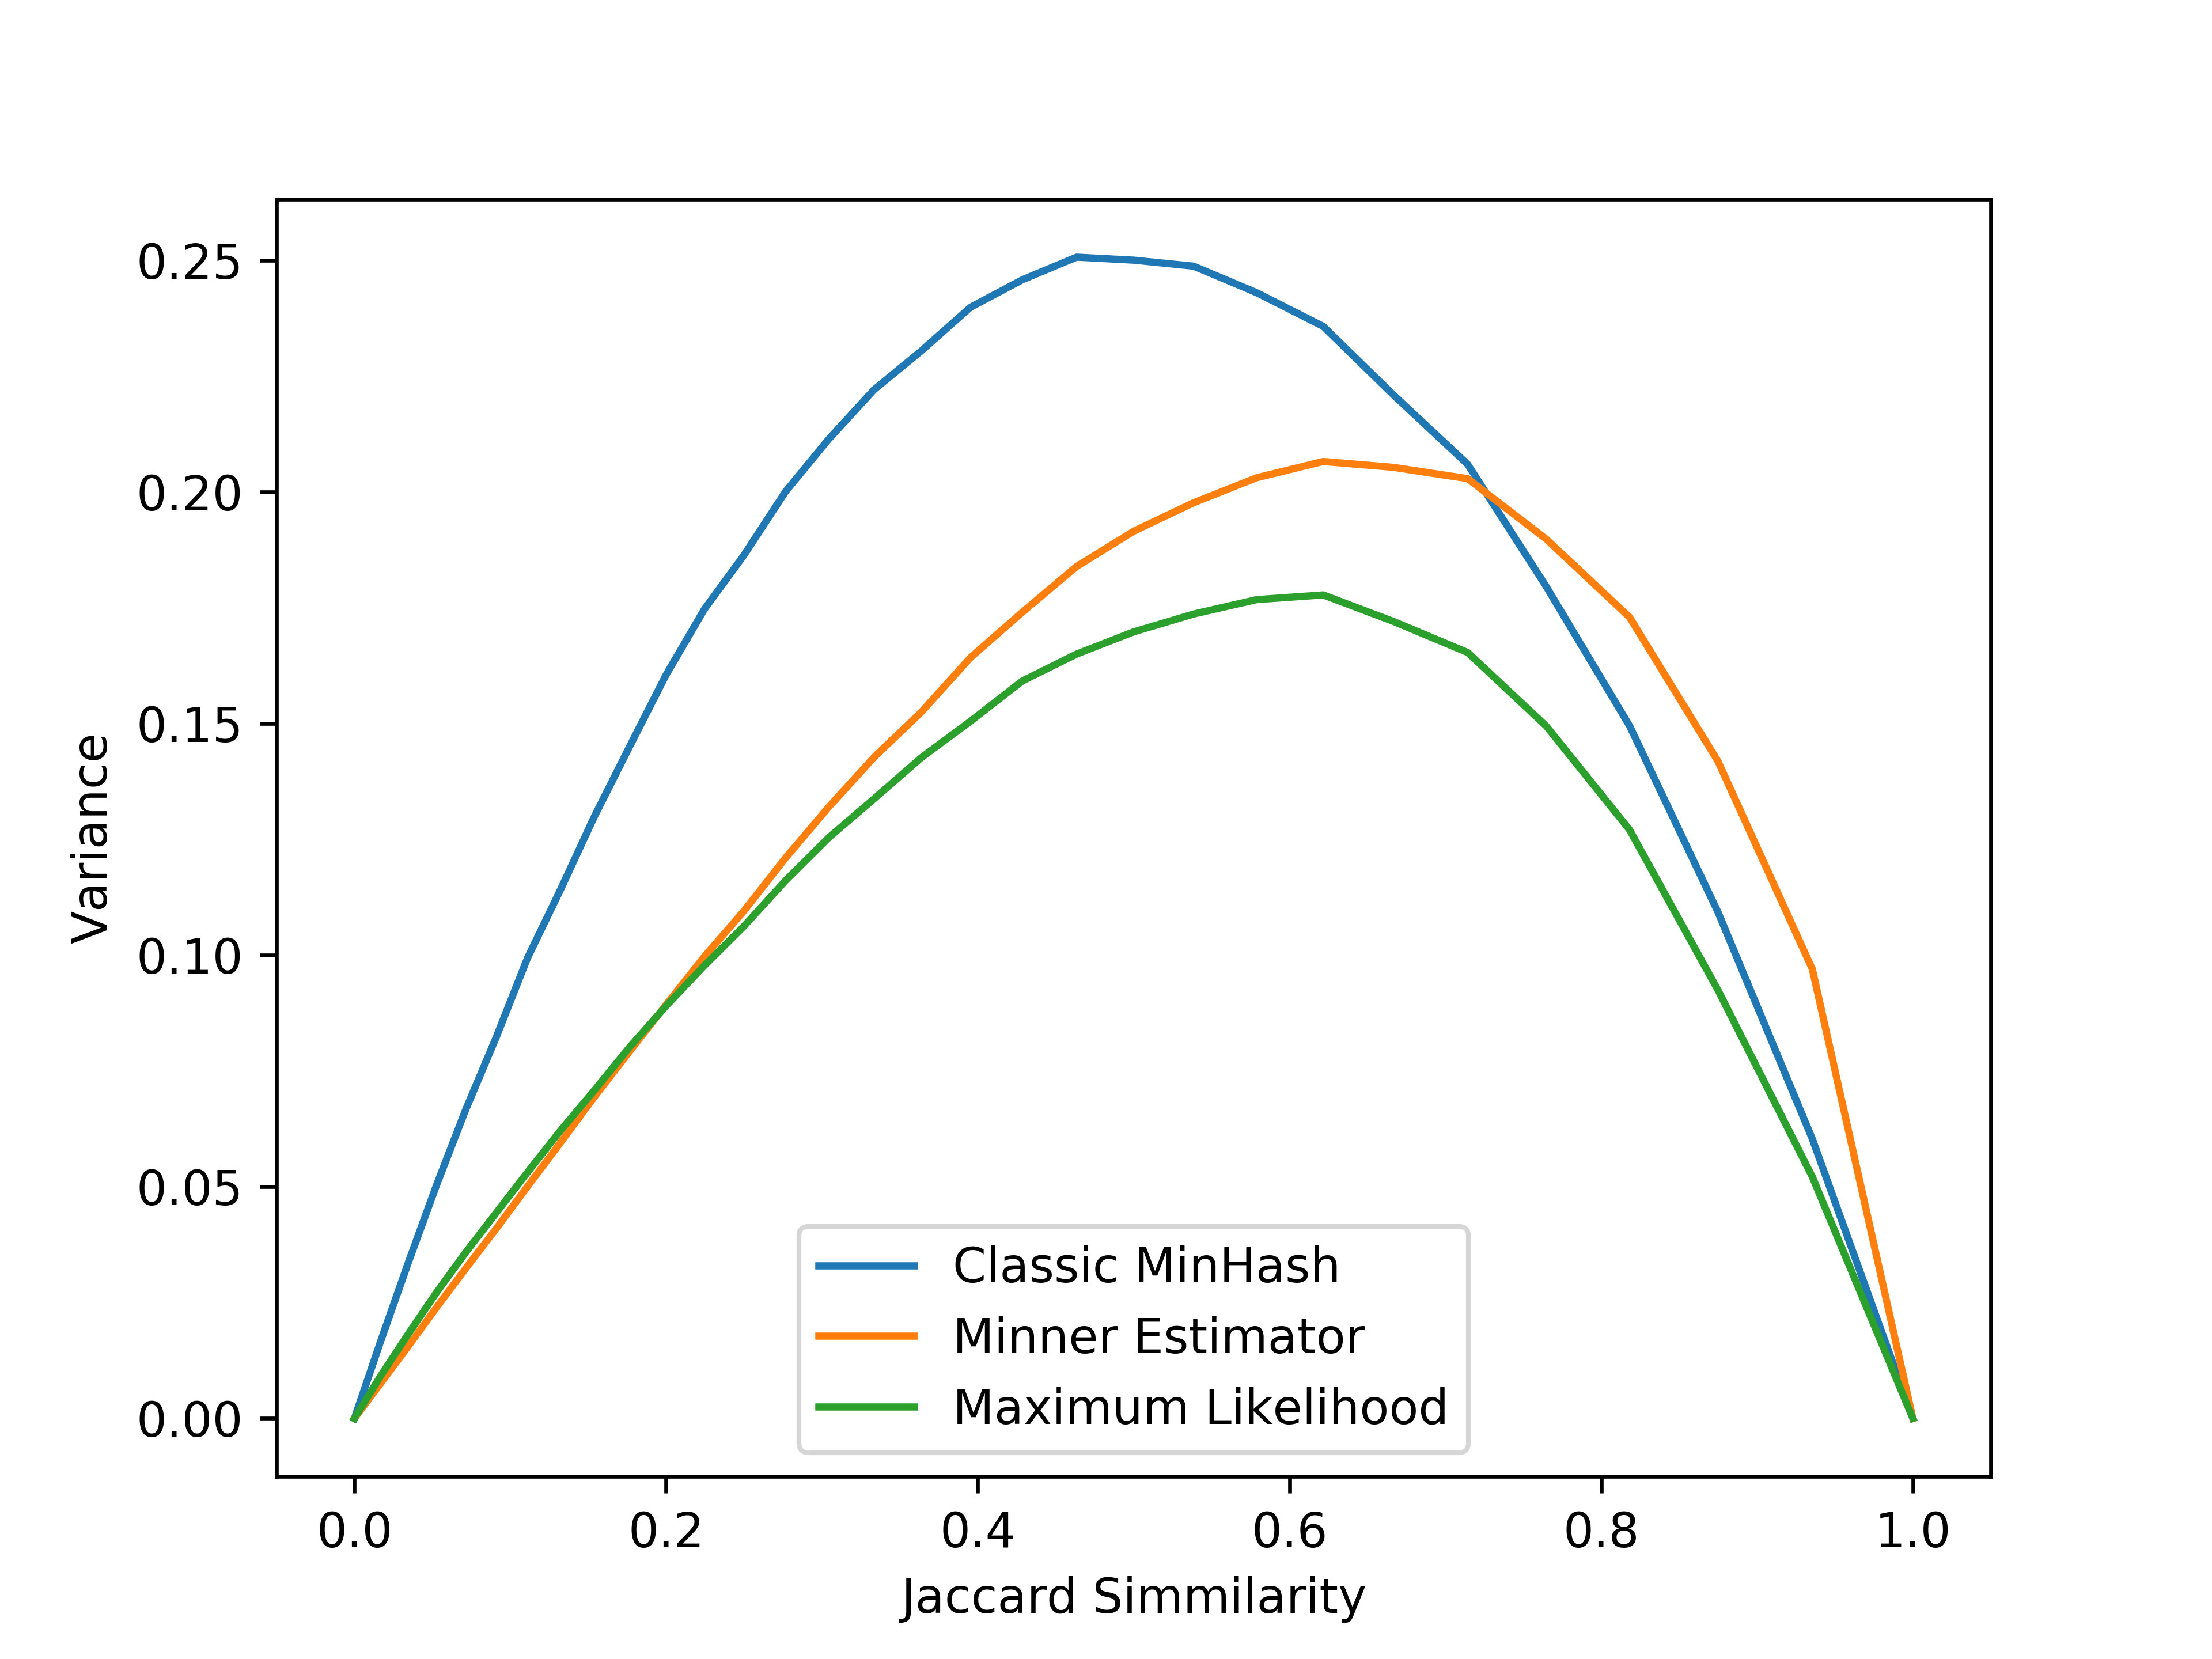
\includegraphics[trim=10 0 45 40,clip,width=\linewidth]{figures/synvar_100000.png}
   \caption{Measured variance of estimators, over 100,000 repetitions at $|X|=|Y|=K=30$ and $u=500$.
      The MLE has already almost converged to \cref{fig:mle_variance}.
      The Minner Estimator is seen to be particular good for low Jaccard similarities, which may be why it works so well on the practical datasets tested in \cref{sec:evaluation} which tend to have similarities concentrated in the $[0,0.2]$ range, as seen in \cref{fig:scatter}.}
   \label{fig:exp_variance}
\end{figure}

In the previous sections we derived and analysed a Jaccard similarity estimator based on maximum likelihood.
The estimator has to evaluate the log-likelihood function, $\ell$, for all $v\in[\min\{n_x,n_y\}+1]$, which means it takes time at least $\Omega(K\min\{n_x,n_y\})$ per database point.

In this section we investigate numerical methods for speeding up the MLE and suggests a new, very fast, estimator we call the Minner Estimator, which can be computed as fast as the classical MinHash estimator.

The starting point of this derivation is the continuous derivative log-likelihood \cref{eq:deriv1},
which we would like to solve $=0$ for $v$.
If we apply the approximation $\log(1-\eps) \approx -\eps$,
we we get
\[
   \frac{d}{dv}\ell(r;v) \approx
   -\frac{[y^*\not\in X]}{n_y-v} 
   -\frac{m}{n_x-v} 
   +\frac{[y^*\in X]}{v} 
   +\frac{r-m}{u-n_x-n_y+v} 
   %= 0
   .
\]
This is a convenient form, since it is linear in the variables, $[y^*\in X]$, $m$ and $r$.
As we observe multiply $r_i$ values, we can define
$R = \sum_i r_i$, $M = \sum_i m_i$ and $C = \sum_i [y_i^*\in X]$.
This gives us a single equation to solve
\[
   \sum_i\frac{d}{dv}\ell(r_i; v) \approx
   -\frac{K-C}{n_y-v} 
   -\frac{M}{n_x-v} 
   +\frac{C}{v} 
   +\frac{R-M}{u-n_x-n_y+v} 
   = 0
   .
   \label{eq:d1_simple}
\]
This equation can be rewritten as a degree three polynomial and solved by standard methods.
The time complexity has thus been decreased from $\Omega(K\min\{n_x,n_y\})$ to $O(K)$ plus the time it takes to find the polynomial roots.

However, solving a polynomial for every point in the database is hardly as fast as the classical MinHash estimator.

However, we would like a simpler estimator still.
In practice $u$ is very large (otherwise it wouldn't be set data), so we'll approximate $\frac{R-M}{u-n_x-n_y+v}\approx 0$.
If we assume $n_y>\!>v$ we may approximate $\frac{K-C}{n_y-v}\approx 0$ we get the simple solution to \cref{eq:d1_simple}, $v=\frac{C n_x}{C+M}$.
Alternatively, if $n_x>\!>v$ we approximate $\frac{M}{n_x-v}\approx 0$, we get $v=\frac{C n_y}{K}$.
We then combine the two approximations into the following estimator:
\begin{definition}[Minner Estimator]
\[
   T_v(r) = \min\left\{\frac{C n_x}{C+M}, \frac{C n_y}{K}\right\}.
   \label{eq:minner}
\]
\end{definition}

The resulting value is clearly always in the acceptable range $[0,\min\{n_x, n_y\}]$, since $C\le C+M$ and $C \le K$.
To estimate Jaccard we take $T_j(r) = v/(n_x + n_y - v)$.
As before we can compute $C$ and $M$ in $O(K)$ time per database point, and now we have replaced the finalization of finding the roots of a polynomial with a simple division.

\hspace{.2em}

While $E[\frac{C n_y}{K}] = v$ is nice and unbiased (for estimating $v$), the combined estimator is not necessary so.
Using the arguments from the previous analysis section, we find that for a single observation,\footnote{We were not able to analyse the case where $C$ and $M$ are the sum of multiple $c_i$ and $m_i$ values, nor the effect of combining the two estimators using the minimum.}
\begin{align}
   E[\frac{c n_x}{c+m}]
   &= \frac{v n_x}{y} E[\frac{1}{1+m}]
   = \frac{v n_x}{n_x-v+1} (H_{n_x+n_y-v} - H_{n_y-1})
 \\&\approx \frac{v n_x}{n_x-v+1} \log\frac{n_x+n_y-v}{n_y-1},
 \label{eq:minner_mean}
\end{align}
where $H_n$ is the $n$th Harmonic Number.
If we let $n_x=n_y=n\to \infty$ we get $\eqref{eq:minner_mean} = \frac{2j}{1-j}\log\frac{2}{1+j}$, a quantity sandwiched between the Jaccard similarity, $j$, and the Sørensen–Dice coefficient, $\frac{2j}{1+j}$.
While not unbiased, this is at least monotone in $j$ (respectively $v$).

Experimentally, the actual Minner Estimator seems to converge to $j$ for larger $K$, at least for the smaller $j$ seen in practice. See~\cref{fig:var}.
For larger Jaccard similarities it slightly underestimate them, just as we see on the variance get worse as $j\to1$ in~\cref{fig:exp_variance}.

\hspace{.2em}

We finally present a numerical way to combine the speed of the Minner Estimator with the consistency of the MLE.
The idea is a common one in MLE design, which is to apply Newton's method to the problem of solving $\frac{d}{dv}\ell(r;v)=0$.%
\footnote{People sometimes use Newton's method with the expected Hessian instead of the actual second derivative~\cite{longford1987fast}, however in our case we'll be able to efficiently compute it exact.}
To maintain $O(K)$ complexity per database point we apply Newton's method to the approximate derivative equation \cref{eq:d1_simple}.
This is nice, because the second derivative is still linear in $C$, $R$ and $M$:
\[
   \sum_i\frac{d^2}{dv^2}\ell(r_i; v) \approx
   \frac{K-C}{(n_y-v)^2} 
   +\frac{M}{(n_x-v)^2} 
   +\frac{C}{v^2}
   +\frac{R-M}{(u-n_x-n_y+v)^2}
   .
   \label{eq:d2_simple}
\]
Newton's method now proceeds with iterations
$v_{i+1} = v_i - \frac{\ell'(r; v_i)}{\ell''(r; v_i)}$.

This concludes the derivation of the Minner Estimator with Newton refinement.
In the next section we give pseudo-code matching what was used to perform our experiments on real world data.

